\documentclass[a4paper,12pt,twoside]{article}%twoside
\usepackage[utf8]{inputenc}
\usepackage[dutch]{babel}
\usepackage{fancyhdr, amsmath, color, graphicx, enumitem, tabularx, hyperref, longtable, multirow, placeins, apacite, subcaption,marvosym,multicol}
\usepackage[framemethod=tikz]{mdframed}
 \usetikzlibrary{positioning}
  \usepackage[margin=2.5cm,headheight=68pt]{geometry}
 %\usepackage[total={16cm, 22cm}]{geometry}
 
\pagestyle{fancy}
\fancyhf{}
\fancyhead[LE,RO]{}%'E': even page, 'O': odd page
\fancyhead[RE,LO]{Correctiesleutels bij oefeningen op flux, inductiespanning en inductiestroom}
\fancyfoot[C]{K. Truyaert}
\fancyfoot[LE,RO]{5TW Toegepaste fysica       \thepage}
%\renewcommand{\labelitemi}{$\circ$}
 
\definecolor{CVO}{RGB}{232, 0, 97}
\setlength\parindent{0pt}

 %Strikeout and highlight text
  \usepackage{soul}
  \usepackage{tikz} % only to get \foreach
  
  %\definecolor{yellow}{RGB}{255,255,0}
  \sethlcolor{yellow}
 
 \begin{document}
\underline{Oefening 6}\newline	Een rechte geleider van 0,500~m lengte wordt met een snelheid van 2,00~m/s doorheen een homogeen magnetisch veld bewogen loodrecht op de veldlijnen. Hierdoor ontstaat tussen de uiteinden van de geleider een inductiespanning van 3,00~V. 
Bereken de grootte van de magnetische veldsterkte van dit magnetisch veld.\\

\underline{Gegeven:}\newline
l = 0,500~m\\
v = 2,00~m/s\\
U$_i$ = 3,00~V\\
\\
\underline{Gevraagd:}\\
B\\ \\
\underline{Oplossing:}\\
In deze vraag beweeg je een rechte geleider loodrecht op een magnetisch veld. Deze situatie gebeurt in onderstaande afbeelding, waar de staaf van links naar rechts  door het magnetisch veld beweegt:
\begin{figure}[h]
	\centering
	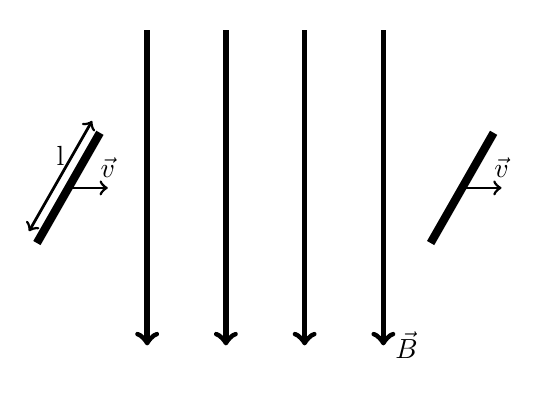
\begin{tikzpicture}
		\draw[->,line width = 2pt] (4,2)--(4,-2) node[right]{$\vec{B}$};
		\draw[->,line width = 2pt] (1,2)--(1,-2);
		\draw[->,line width = 2pt] (2,2)--(2,-2);
		\draw[->,line width = 2pt] (3,2)--(3,-2);
		\draw[-,line width = 3pt] (-0.4,-0.7)--(0.4,0.7);
		\draw[<->,line width = 1pt] (-0.5,-0.55)--(0.3,0.85) node[midway,above]{l};
		\draw[->,line width = 1pt] (0,-0)--(0.5,0) node[above] {$\vec{v}$};
		\draw[-,line width = 3pt] (4.6,-0.7)--(5.4,0.7);
		\draw[->,line width = 1pt] (5,-0)--++(0.5,0) node[above] {$\vec{v}$};
	\end{tikzpicture}
\end{figure}

De grootte van het magnetisch veld kan je via het inductieverschijnsel in een rechte, bewegende geleider vinden. Hiervoor gebruik je de vergelijking:\[\left|U_i\right|= NBlv.\]
Deze vergelijking omvormen naar $B$ levert de volgende vergelijking op:
\[B = \frac{\left|U_i\right|}{Nlv}.\]
Invullen van alle gekende factoren (N=1), levert een magnetische veldsterkte vn 3,00~T op.


\newpage






\underline{Oefening 7}\newline	We trekken een rechte draad van 50,0~cm lang, die deel uitmaakt van een stroomkring met totale weerstand 0,0100~$\Omega$, met een snelheid van 5,00~m/s doorheen een homogeen magnetisch veld met veldsterkte 0,700~T. Bewegingsrichting, draad en magnetische veldlijnen staan loodrecht op elkaar. 
Bereken tijdens deze beweging :
\begin{enumerate}
	\item de inductiespanning
	\item	de inductiestroom
	\item	de kracht die de draad vanwege het magnetisch veld ondervindt
\end{enumerate} 

\underline{Gegeven:}\newline
l = 0,500~m\\
v = 5,00~m/s\\
R = 0,0100~$\Omega$\\
B = 0.700~T
\\ \\
\underline{Gevraagd:}
\begin{enumerate}
	\item U$_i$
	\item I$_i$
	\item F
\end{enumerate} 
\underline{Oplossing:}\\
\begin{enumerate}
	\item In deze vraag beweeg je een rechte geleider loodrecht op een magnetisch veld. Deze geleider is een halve meter lang en is onderdeel van een grotere stroomkring. De inductiespanning bepaal je opnieuw via de vergelijking van het inductieverschijnsel in een rechte, bewegende geleider vinden:\[\left|U_i\right|= NBlv.\]
	In dit geval levert dat dus een inductiespanning van $\left|U_i\right| = 1,75~V$ op.
	\item Deze spanning zal dus door de stroomkring lopen. De weerstand van die stroomkring is gekend. Via de wet van Ohm kan je dus de waarde van de inductiestroom gaan bepalen:
	\[I_i = \frac{U_i}{R} = 175~A.\]
	\item De kracht op de bewegende geleider bepaal je via de Lorentzkracht:\[F = BIl = 61,3~N.\]
\end{enumerate}
\newpage


\underline{Oefening 8}\newline	Een magnetisch veld met lengte 240~cm verdwijnt loodrecht in het vlak van dit blad. Een blokje met lengte l beweegt rechtlijnig naar rechts door dit veld met snelheid v. De magnetische flux door het blokje wordt gedurende deze beweging voorgesteld als functie van de tijd in de rechtergrafiek.
\begin{enumerate}
	\item Bereken de lengte van het blokje.
	\item Met welke snelheid beweegt het blokje?
\end{enumerate} 

\underline{Gegeven:}\newline
d = 2,40~m\\

\underline{Gevraagd:}
\begin{enumerate}
	\item l
	\item v
\end{enumerate} 
\underline{Oplossing:}\\
In deze vraag beweeg je een rechthoekig blokje loodrecht op een magnetisch veld. Dit magnetisch veld is uitgespannen over een lengte $d$. Deze geleider beweegt zich in het magnetisch veld tussen $t=2~s$ en  $t=4~s$. Daarna is de maximale flux bereikt en blijft deze behouden tot $t= 10~s$. De flux wordt daarna terug kleiner, aangezien de rechthoekige geleider zich in een tijdspanne van 2 seconden uit het magnetisch veld verwijdert. \\
De geleider doet er dus 2 seconden over om zijn volledige lengte af te leggen, aangezien de maximale flux na 2 seconden bereikt wordt. We weten dus dat, aglemeen, $\Delta s = v\Delta t$, ofwel dat in dit geval geldt dat $l = v\cdot 2~s$.\\
Nu het blokje volledig in het magnetisch veld hangt, blijft de flux tussen $t=4~s$ en $t=10~s$ constant. In die tijdspanne legt het blokje opnieuw een afstand $\Delta s$, nu gelijk aan $v\cdot 6~s$ af, die ditmaal gelijk is aan 2,40~m-l, zoals te zien is in onderstaande figuur:
\begin{figure}[!h]
	\centering
	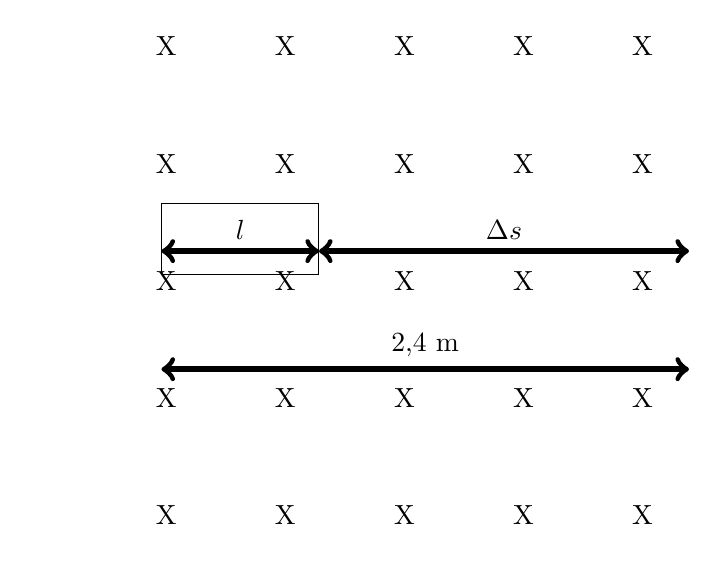
\begin{tikzpicture}
	\node[white] (n00) {X};
	\foreach \x [remember=\x as \lastx (initially 0)] in {0,...,4}{
		\node[right =of n\lastx0] (n\x0) {X};
		\foreach \y [remember=\y as \lasty (initially 0)] in {1,...,4}{
			\node[below =of n\x\lasty] (n\x\y) {X};
		}
	}
	\draw(1.45,-2.9) rectangle (3.45,-2);	
	\draw[<->, line width = 2pt](1.45,-4.1) --++ (6.7,0) node[midway,above]{2,4~m};		
	\draw[<->, line width = 2pt](3.45,-2.6) --++ (4.7,0) node[midway,above]{$\Delta s$};		
	\draw[<->, line width = 2pt](1.45,-2.6) --++ (2,0) node[midway,above]{$l$};		
	\end{tikzpicture}
\end{figure}
We weten dus dat enerzijds $l = 2~s\cdot v$ en anderzijds dat $2,40~m=l+6~s\cdot v$. Na substitutie vind je dat $v = 0,3~m/s$ en dat $l=0,60~m$.








 \end{document}
